\section{Preliminary Results}
\label{sec-results}

To collect spectrum utilization information, Wifi cards needs to be put in
monitor mode so that every decoded packet are delivered to upper layer.
However, almost none of current smartphone hardwares support monitor mode natively,
at least without firmware and driver hacking. To mitigate this limitation, we
use external Wifi dongle to mimic future smartphones hardwares with built-in
monitor mode support. Table~\ref{tab:dongle} shows the specification of the Wifi
dongle used in our experiments. The dongle is connected to smartphones through
OTG cable. We refer a smartphone with Wifi dongle as \textit{sniffer device}
hereafter.

\begin{table}[t!]
  \centering
  \begin{tabular}{ll}
    \toprule
    \textbf{Model} & ALFA Network AWUS036H \\
    \textbf{Chipset} & RTL8187L \\
    \textbf{Connector} & $1\times2.4$GHz SMA \\
    \textbf{Antenna} & 2.5dBi rubber duck \\
    \textbf{Wifi Support} & 802.11b/g \\
    \bottomrule
  \end{tabular}
  \caption{Wifi dongle specification.}
  \label{tab:dongle}
\end{table}


\subsection{Rogue Access Point}

Rogue Access Point (RAP) are unauthorized APs that connected to secure corporate
network. They pose security vulnerabilities as well as undesired Radio Frequency
(RF) interferences to (usually) well planed corporate networks. Most
RAPs are set up by employees for their own convenience. Thus besides being able to
simply detect the existence of RAPs, it's also interesting to see the impact the
RAPs: how many devices the RAP serve and how much traffic it
generates. These information helps the network administrator to decide
undeserved areas and improve spatial planing.

In this experiment, we recruited volunteers whose office or laboratory are in
the same campus building, and equipped them with sniffer device which are put in
monitor mode. Each volunteers carries the device as they conduct their
daily work routine. In total, 38 device-hour's data (contains 37M packets) are
captured.  We identify RAPs by inspecting beacon frames and excluding campus APs
and temporary hotspots that only exist for a short period of time. 11 RAPs were
identified, and Figure~\ref{fig:rap} shows the traffic volume generated by these
RAPs as well as number of devices that ever connected to these RAPs.

\begin{figure}[t!]
  \centering
  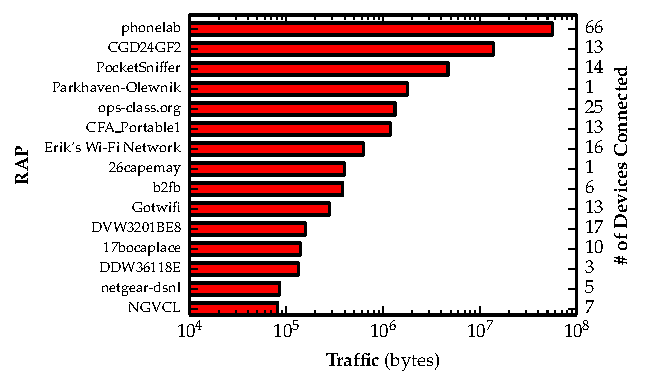
\includegraphics[width=0.48\textwidth]{./figures/RAPTrafficGraph.pdf}
  \caption{Rogue AP traffic detected by sniffer device.}
  \label{fig:rap}
\end{figure}

Among the detected RAPs, \texttt{phonelab} and \texttt{ops-class.org} are known
to be open access APs set up by the authors.  They both generate a large amount of
traffic and serve a fair large number of devices, which indicates potential coverage
holes of the campus network. Another RAP, \texttt{Parkhaven-Olewnik}, also
generated huge traffic yet all of them are with one device. This indicates a
typical personal RAPs that are used and secured by the owner.


\subsection{Channel Assignment}
To demonstrate the feasibility of using client-side measurements to improve
channel assignment, we built an concept-proof system, where a sniffer device,
when connected to \PS{}-enabled APs, will periodically collect
and report the traffic condition, so that the AP can determine the least
congested channels based on the feedback of all associated devices. 

The experiment is designed as follows. We first set up \texttt{iperf} UDP
traffic between \PS{}-AP $A$ and sniffer device $D_1$ on channel $C_1$ at a
constant data rate (15 Mbits/s). Then another device, $D_2$, starts jamming the
channel by sending saturated UDP traffic. Since $D_1$ periodically collects and
reports traffic information, $A$ will eventually realize this interference and
find another less congested channel $C_2$ and switch to it. Figure~\ref{fig:bw}
shows the bandwidth change of the link between $A$ and $D_1$. We conduct the
experiment at 2.4GHz band and in this particular run, $C_1$ is channel 11 and $C_2$
is channel 1.

At 8.5s, when $B$ starts jamming the channel, the link bandwidth between $A$ and
$D_1$ decreased and fluctuated due to the interference, then at 75s, when $A$
and $D_1$ switch to a less congested channel, the bandwidth resumes up to
previous level before the interference.

\begin{figure}[t!]
  \centering
  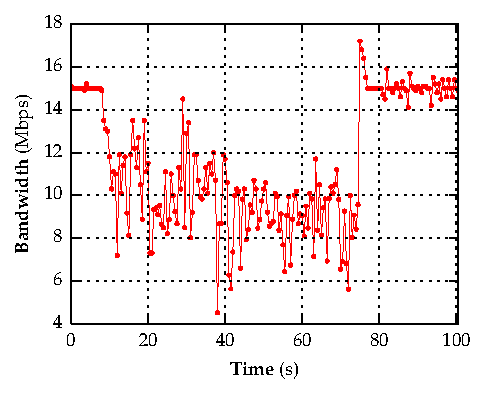
\includegraphics[width=0.48\textwidth]{./figures/ChannelBWGraph.pdf}
  \caption{Bandwidth change after jamming and channel switch.}
  \label{fig:bw}
\end{figure}
